\chapter{Narukvica}
\label{pog:bracelet}
Svrha narukvice je prikupljanje biomedicinskih parametara korisnika i njihovo slanje na obradu na glavnoj ploči. Biomedicinski parametri koji će se promatrati su brzina otkucaja srca putem fotopletizmografskog senzora (PPG) i impedancija kože, odnosno elektrodermalna aktivnost. 

Što se tiče zahtjeva na napajanje narukvice, situacija je ista kao i kod glavne ploče, uz drugačiju potrošnju. Tako da izrada pločice za narukvicu predstavlja mogućnost ispravljanja grešaka nastalih tijekom dizajna napajanja glavne ploče. Narukvica također mora imati mogućnost bežične komunikacije. S obzirom na ograničenje veličine ploče maknuti su kratkospojnici i testne točke.

\section{Bežična komunikacija}
Shema bežične komunikacije na narukvici (slika \ref{slk:BR_WIRELESS}) je veoma slična onoj na glavnoj ploči (slika \ref{slk:WIFI}), uz nedostatak kratkospojnika, dodatak signala za upravljanje I\textsubscript{2}C sučeljem i korištenje analogno-digitalnog pretvornika za mjerenje impedancije kože. Još jedna promjena dolazi u obliku programiranja preko UART-a. S obzirom na probleme tijekom programiranja glavne ploče dodani su signali DTR i CTS kako bi se BOOT i EN stezaljke ESP mikrokontrolera mogle programski upravljati.
\begin{sidewaysfigure}[htbp]
    \centering
    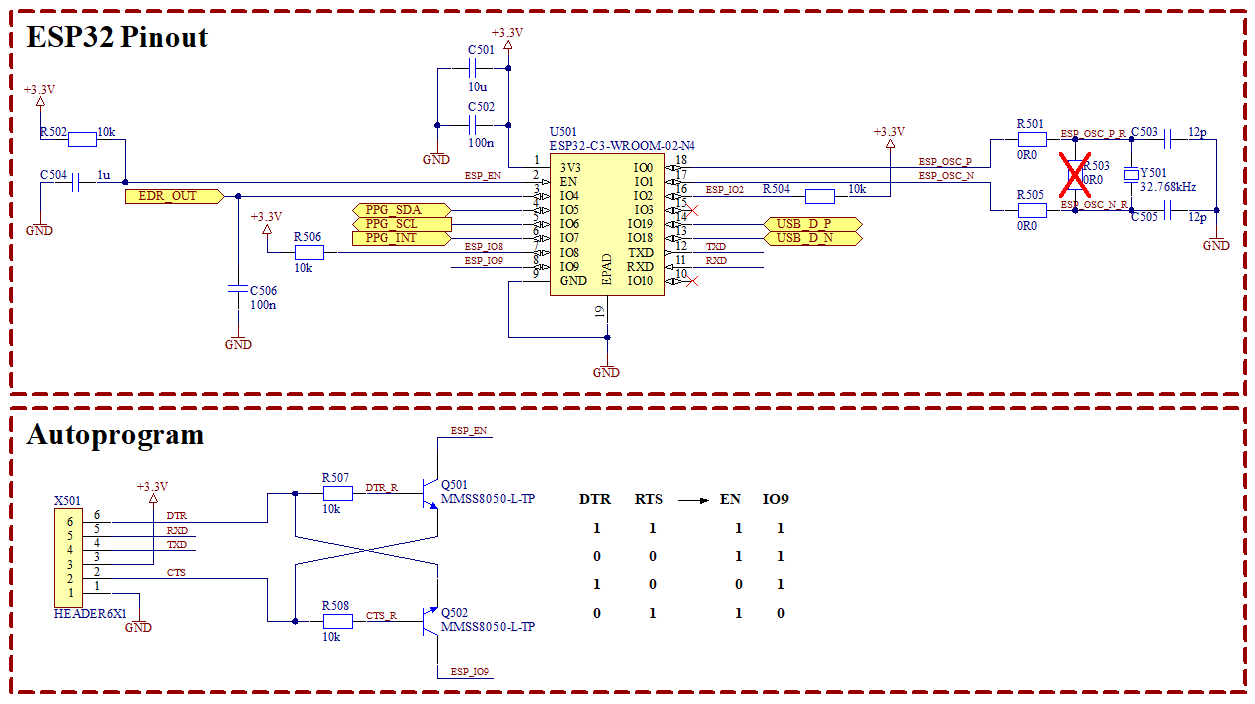
\includegraphics[width=1\textwidth]{Figures/BR_WIRELESS.png}
    \caption{Shema bežične komunikacije narukvice}
    \label{slk:BR_WIRELESS}
\end{sidewaysfigure}

\newpage
\section{Fotopletizmografski senzor}

Za mjerenje brzine otkucaja srca koristi se PPG senzor MAX30101 tvrtke Analog Devices (slika \ref{slk:MAX30101}). Ovaj senzor u sebi ima crvenu, zelenu i infracrvenu svjetleću diodu i fotosenzor, upravljačko sklopovlje za diode, te komunicira preko I\textsuperscript{2}C sučelja. Kao što je vidljivo na shemi na slici \ref{slk:PPG} ovaj senzor je veoma jednostavan za implementaciju uz svega par par priteznih otpornika i blokadnih kondenzatora. Jedina komplikacija dolazi u obliku napajanja od 5 V, koje je potrebno jer je pad napona na zelenoj svjetlećoj diodi specificiran na 3.3 V.
\begin{figure}[htb]
    \centering
    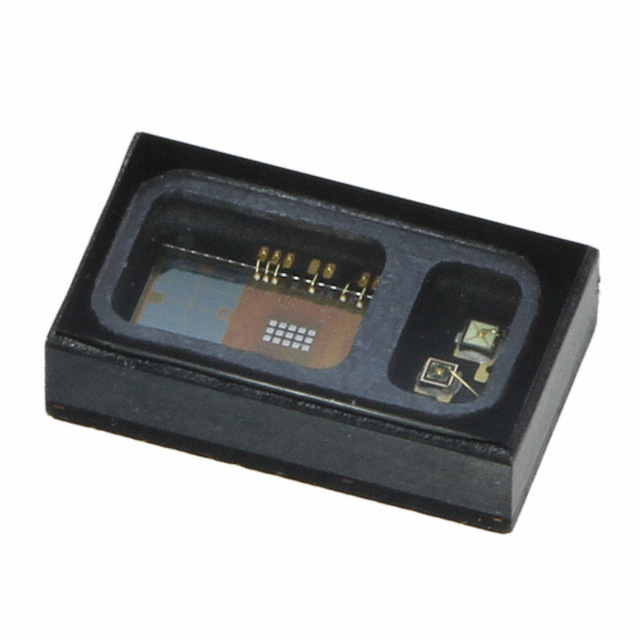
\includegraphics[width=6 cm]{Figures/MAX30101.JPG}
    \caption{MAX30101 PPG senzor}
    \label{slk:MAX30101}
\end{figure}
\begin{figure}[htb]
    \centering
    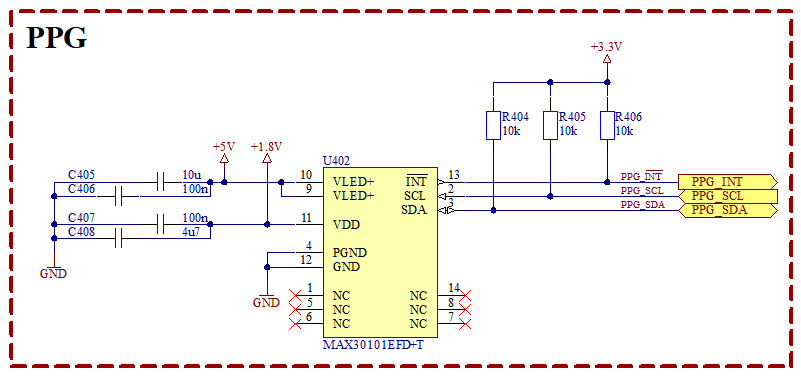
\includegraphics[width=\textwidth]{Figures/PPG.png}
    \caption{Shema PPG senzora}
    \label{slk:PPG}
\end{figure}

\section{Impedancija kože}
Impedancija kože mjerit će se pomoću instrumentacijskog pojačala. Shema mjernog kruga prikazana je na slici \ref{slk:EDR}. Odabrano je instrumentacijsko pojačalo AD8226 tvrtke Analog Devices zbog svog velikog ulaznog otpora, malog šuma i dobrog potiskivanja zajedničkih smetnji \cite{ad:ad8226}. Napajanje pojačala je filtrirano pasivnom mrežom kako ne bi došlo do smetnji od digitalnog dijela sklopovlja.
\begin{figure}[htb]
    \centering
    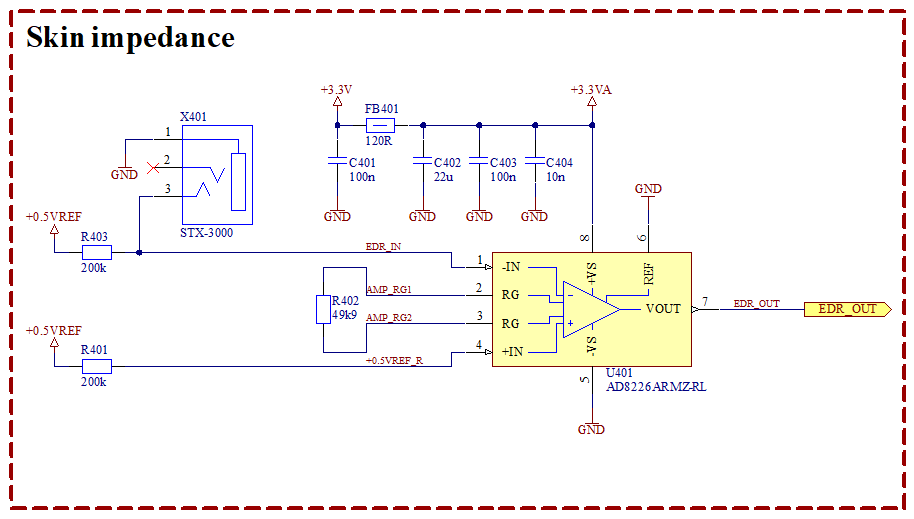
\includegraphics[width=\textwidth]{Figures/EDR.png}
    \caption{Shema mjernog kruga za impedanciju kože}
    \label{slk:EDR}
\end{figure}
Za mjerenje impedancije koristi se referentni napon od 0.5 V, a mjerenje impedancije se temelji na mjerenju napona na naponskom djelilu na stezaljci -IN pojačala. Kožu predstavlja donji otpornik u naponskom djelilu, te razlika između tog napona i referentnog napona pojačava:
\begin{equation} \label{eq:EDR}
    U_{IZ}=A\cdot U_{REF}\cdot \frac{R_{403}}{R_{403}+R_{skin}}
\end{equation}
Impedancija kože mjeri se u stotinama kilooma (maksimalno cca. $250\textrm{ k}\Omega$ \cite{rskin}), tako da je vrijednost gornjeg otpornika $200\textrm{ k}\Omega$. Pojačanje iznosi 2 i namješta se preko otpornika R402.

Za svrhe lakšeg prototipiranja koristit će se samoljepljive elektrode (slika \ref{slk:ELECTRODE}) koje se montiraju na kabel prikazan na slici \ref{slk:CABLE}. 
\begin{figure}[htb]
    \centering
    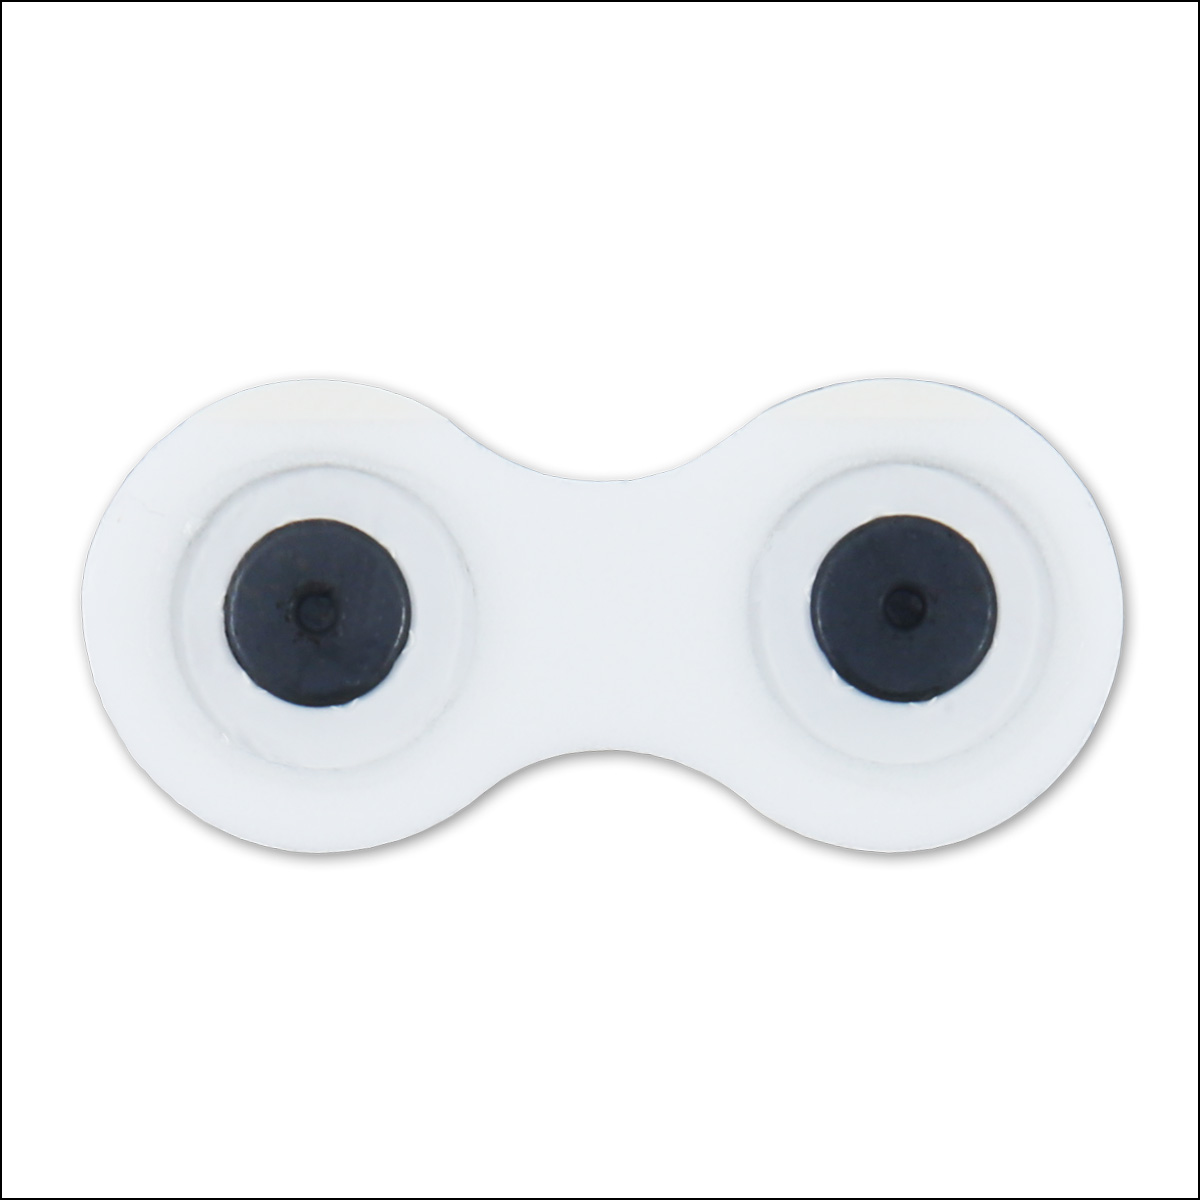
\includegraphics[width=6 cm]{Figures/ELECTRODE-BOTTOM.jpg}
    \caption{Samoljepljiva elektroda}
    \label{slk:ELECTRODE}
\end{figure}
\begin{figure}
    \centering
    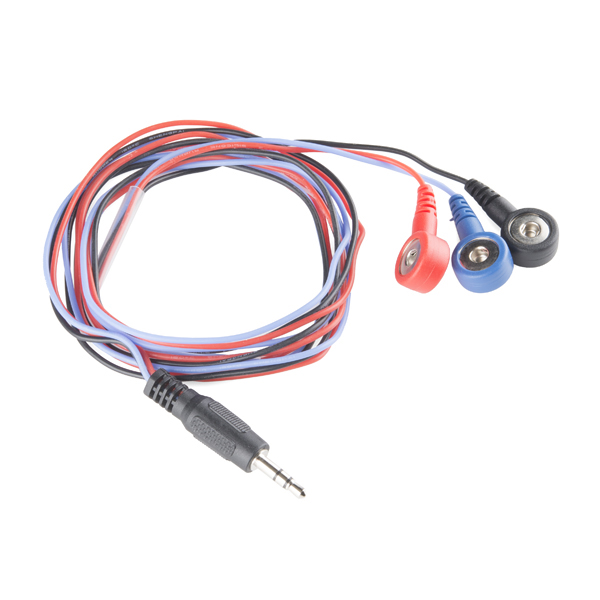
\includegraphics[width=6 cm]{Figures/CABLE.jpg}
    \caption{Kabel za elektrode}
    \label{slk:CABLE}
\end{figure}
Ovaj kabel se spaja na narukvicu putem 3.5 mm audio priključka.

\section{Napajanje}
\subsection{Proračun potrošnje}

Proračun potrošnje za narukvicu je bio puno jednostavniji od proračuna za glavnu ploču. U ovom slučaju, najveći potrošač je i dalje sustav za bežičnu komunikaciju, međutim on je efektivno i jedini potrošač na 3.3 V jer je potrošnja instrumentacijskog pojačala izrazito mala, maksimalno 20 $\mu\textrm{A}$ \cite{ad:ad8226}. Za potrošnju sustava bežične komunikacije uzima se vrijednost prikazana u tablici \ref{tab:MB3V3}. Na napajanju od 5 V jedini potrošač je PPG senzor i njegova potrošnja u najgorem slučaju iznosi 50 mA, a na napajanju od 1.8 V senzor troši maksimalno 1.1 mA \cite{ad:max30101}.

\subsection{Napajanja od 3.3 V i 1.8 V}
\label{subsec:BR_VDD}
Shema napajanja od 3.3 V i 1.8 V prikazana je na slici \ref{slk:BR_VDD}. U oba slučaja koristi se LDO AP2112K proizvođača Diodes Incorporated. Ovaj LDO je odabran radi svoje male veličine u SOT-25 s obzirom na ograničenje veličine PCB-a.
\begin{figure}[htb]
    \centering
    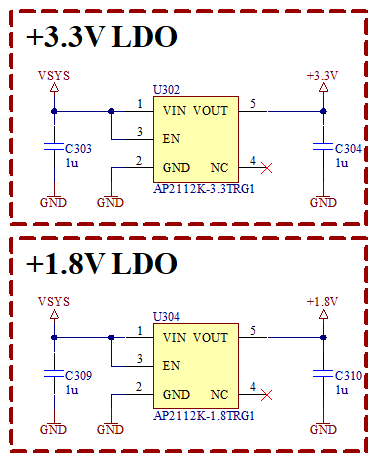
\includegraphics[width=6 cm]{Figures/BR_VDD.png}
    \caption{Napajanje od 3.3 V i 1.8 V za narukvicu}
    \label{slk:BR_VDD}
\end{figure}

\subsection{Referentni napon}

Shema izvora referentnog napona prikazana je na slici \ref{slk:BR_VREF}. Koristi se ADR130 referenca tvrtke Analog Devices. Iznos referentnog napona se može namjestiti na 1 V ili 0.5 V, a veličina kućišta je ista kao i kod linearnih regulatora prikazanih u dijelu \ref{subsec:BR_VDD}.
\begin{figure}[htb]
    \centering
    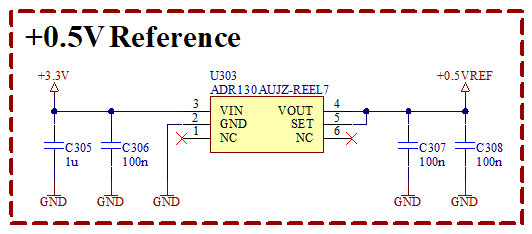
\includegraphics[width=10 cm]{Figures/BR_VREF.png}
    \caption{Referentni izvor napona od 0.5 V}
    \label{slk:BR_VREF}
\end{figure}

\subsection{Napajanje od 5 V}

Za napajanje od 5 V bilo je potrebno dizajnirati uzlazni prekidački regulator. Shema regulatora prikazana je na slici \ref{slk:BR_BOOST}. Odabran je TLV61220 proizvođača Texas Instruments jer je idealan za napajanje s baterije. Regulator može raditi na ulaznom naponu od 0.7 V do 5.5 V i potrebno je malo komponenata za rad \cite{ti:tlv61220}. Također je pogodan radi svoje male veličine u SOT-23 kućištu.
\begin{figure}[htb]
    \centering
    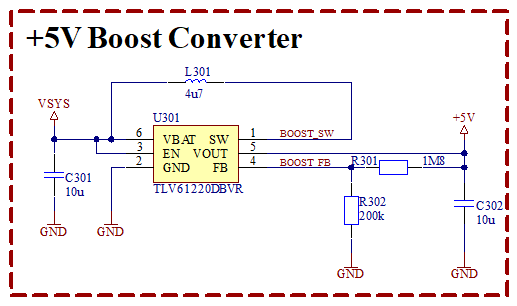
\includegraphics[width=10 cm]{Figures/BR_BOOST.png}
    \caption{Uzlazni prekidački regulator}
    \label{slk:BR_BOOST}
\end{figure}
Zavojnica je odabrana prema preporukama proizvođača, a naponsko djelilo je proračunato imajući na umu da donji otpornik ne bi trebao biti veći od $500\textrm{ k}\Omega$ kako bi vrijednost struje koja teče u FB stezaljku bila što bliže 0.01 $\mu\textrm{A}$ \cite{ti:tlv61220}. Efikasnost za izlazne struje od 1 mA do 50 mA je skoro ista na ulaznom naponu u rasponu baterije i može se uzeti efikasnost od 90 \% (\ref{slk:BOOST_EFF}). Uz minimalni ulazni napon od 3 V, potrošnja, prema jednadžbi \ref{eq:IN_CURR} iznosi 75 mA.
\begin{figure}[H]
    \centering
    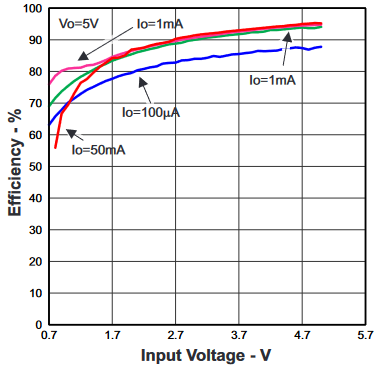
\includegraphics[width=6 cm]{Figures/BOOST_EFF.png}
    \caption{Efikasnost regulatora \cite{ti:tlv61220}}
    \label{slk:BOOST_EFF}
\end{figure}

\section{Baterija i punjač baterije}
\label{sec:BR_BATCHG}
Uzevši u obzir potrošnju svih podsustava ukupna struja koju punjač mora moći dati je 426.12 mA. Uz struju punjenja baterije od 1 A i uzevši u obzir jednadžbe \ref{eq:IN_CURR} i \ref{eq:IN_CURR_MAX} ukupna struja koju USB sučelje mora moći dati iznosi 1.08 A, dakle uzet će se ograničenje na ulaznu struju od 1.5 A. Uvjeti su, dakle, veoma slični onima kao kod glavne ploče.

\subsection{Punjač baterije}
Shema punjača narukvice na slici \ref{slk:BR_BATCHG} veoma je slična shemi sa slike \ref{slk:MB_BATCHG}. Promijenjena je svjetleća dioda za indikaciju punjenja u žutu, kako bi se jasnije mogla razlikovati indikacija između indikacije punjenja i indikacije statusa dobrog napajanja. Također su dodani veći otpornici u seriju s diodama jer je svjetlina bila prevelika.
\begin{figure}[H]
    \centering
    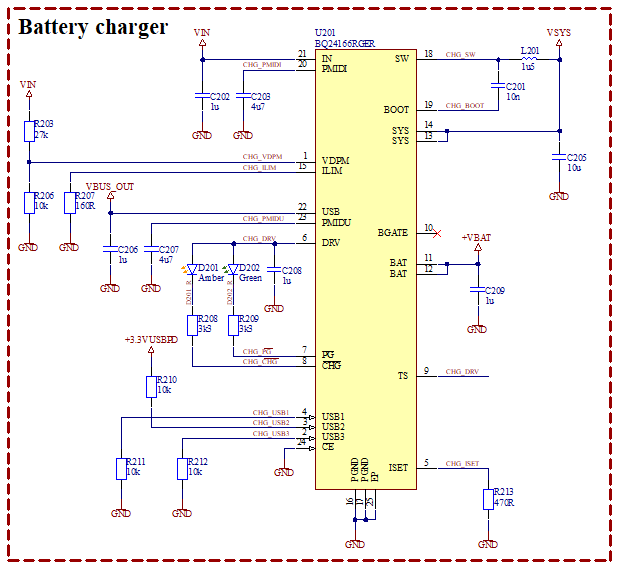
\includegraphics[width=\textwidth]{Figures/BR_BATCHG.png}
    \caption{Shema punjača baterije na narukvici}
    \label{slk:BR_BATCHG}
\end{figure}

Još jedna razlika je u priteznim otpornicima na konfiguracijskim linijama za ograničenje struje USB-a, ovdje je ograničenje uvijek 1.5 A jer nema potrebe za drugačijim postavkama i postoji ograničenje na veličinu pločice. S obzirom na ograničenje na veličinu pločice ovdje je odabrana zavojnica od 1.5 $\mu \textrm{H}$.

Zadnja razlika je vrlo suptilna, ali veoma ključna za ispravan rad punjača. Pogledom na shemu na slici \ref{slk:MB_BATCHG} vidljivo je da stezaljka TS nije nigdje spojena, odnosno ,,pluta''. Ova stezaljka služi za mjerenje temperature baterije tijekom punjenja. Ako je temperatura prevelika ili premala punjenje se zaustavlja. Shema mjerenja prikazana je na slici \ref{slk:BATCHG_TS}. Mjeri se napon na naponskom djelilu kojega čine otpornici i NTC termistor. Naponi na kojima se zaštita aktivira iznose 30\% i 60\% napona na stezaljci DRV, dakle 1.56 V i 3.12 V. S obzirom na to da stezaljka TS ,,pluta'', napon na stezaljci je manji od donjega praga i punjenje ne radi. Kako bi se mjerenje temperature onemogućilo napon na TS stezaljci mora biti veći od 70\% napona na stezaljci DRV. Iz tog razloga proizvođač preporučuje kratko spajanje stezaljka TS i DRV kako bi punjenje cijelo vrijeme bilo omogućeno.
\begin{figure}[htb]
    \centering
    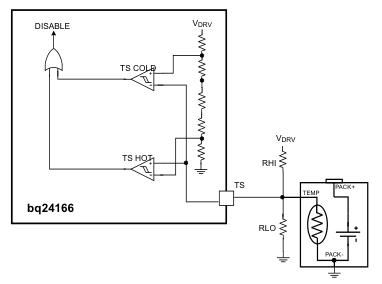
\includegraphics[width=10 cm]{Figures/BATCHG_TS.png}
    \caption{Mjerenje temprature senzora}
    \label{slk:BATCHG_TS}
\end{figure}

\subsection{Baterijska zaštita}
\sloppy Shema baterijske zaštite na narukvici je prikazana na slici \ref{slk:BR_BATPROT}. Shema je slična onoj s glavne ploče na slici \ref{slk:MB_BATPROT}, a ovdje su tranzistori pažljivije odabrani. Maksimalna struja pražnjenja iznosi, prema \ref{sec:BR_BATCHG}, iznosi 426.12 mA. Za aktivaciju zaštite uzet će se struja od $I_{OCD}=1.5\textrm{ A}$, dakle otpor obaju FET-ova prema jednadžbi \ref{eq:TRANCUR} iznosi ${2R_{DS(on)}=66.67\textrm{ m}\Omega}$. Na temelju toga, struja na kojoj će se aktivirati zaštita za punjenje iznosi $I_{OCC}=1.5\textrm{ A}$. Dakle, tranzistor treba imati otpor $R_{DS(on)}=33.33\textrm{ m}\Omega$. Struja na kojoj će se aktivirati zaštita od kratkog spoja iznosi $I_{SCD}=7.5\textrm{ A}$, tako da tranzistor mora moći podnijeti tu struju. Prikaz promjene otpora u ovisnosti o naponu i struji odabranog tranzistora prikazana je na slici \ref{slk:RDS_NEW}. Vidljivo je da će otpor biti veći s većom strujom, što znači da će se zaštita aktivirati nešto prije vrijednosti proračunatih pragova, a opet se neće aktivirati prerano da se onemogući punjenje, što je i poželjno s perspektive sigurnosti.
\begin{figure}[htb]
    \centering
    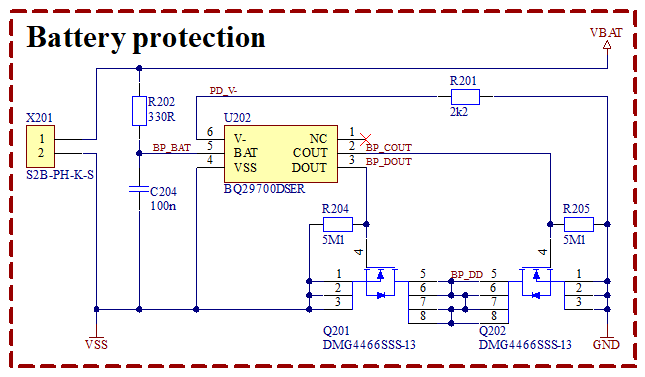
\includegraphics[width=10 cm]{Figures/BR_BATPROT.png}
    \caption{Baterijska zaštita na narukvici}
    \label{slk:BR_BATPROT}
\end{figure}
\begin{figure}[h!tb]
    \centering
    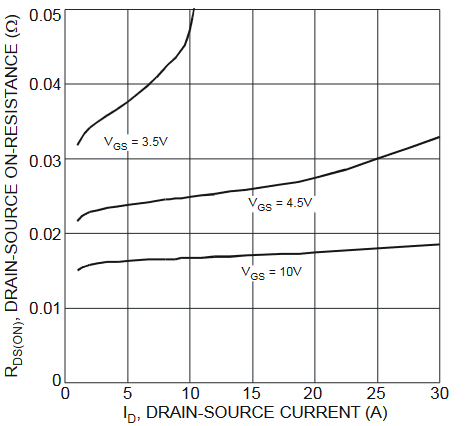
\includegraphics[width=6 cm]{Figures/RDS_NEW.PNG}
    \caption{Graf ovisnosti otpora o naponu između upravljačke elektrode i uvoda tranzistora DMG4466SSS-13 \cite{di:dmg4466}}
    \label{slk:RDS_NEW}
\end{figure}
Očito je da je ovo bolje projektirana zaštita u odnosu na onu na glavnoj ploči.

Ovdje su još dodani i otpori između upravljačke elektrode i uvoda tranzistora koji služe za bolje izbijanje naboja na kapacitetu između upravljačke elektrode i uvoda tranzistora \cite{ti:bq29700}.

\section{USB napajanje}
\label{sec:BR_USB}
Shema USB napajanja narukvice prikazana je na slici \ref{slk:BR_USB}. Dodan je pritezni otpornik R102 koji osigurava da ne dolazi do smanjenja napona na uvodu tranzistora Q101B radi diode u tranzistoru Q101A. Dodana je i Zener dioda od 10 V koja služi za zaštitu od prevelikog napona.

Osim toga, naponska djelila koja služe za podešavanje struje i napona USB-a se sada napajaju s internog regulatora čipa. Kod središnjeg uređaja (slika \ref{slk:MB_USB}) su se napajala s regulatora od 3.3 V koji se nalazi na pločici, što je u redu dok god je prikopčana puna baterija. Međutim, u slučaju prazne ili iskopčane baterije dolazi do problema, jer je sada sustav ostao bez napajanja i ne mogu se podesiti naponi i struje USB-a. To je veoma grub previd i ispravljen je na ovaj način, što je i preporuka proizvođača.
\begin{figure}[htb]
    \centering
    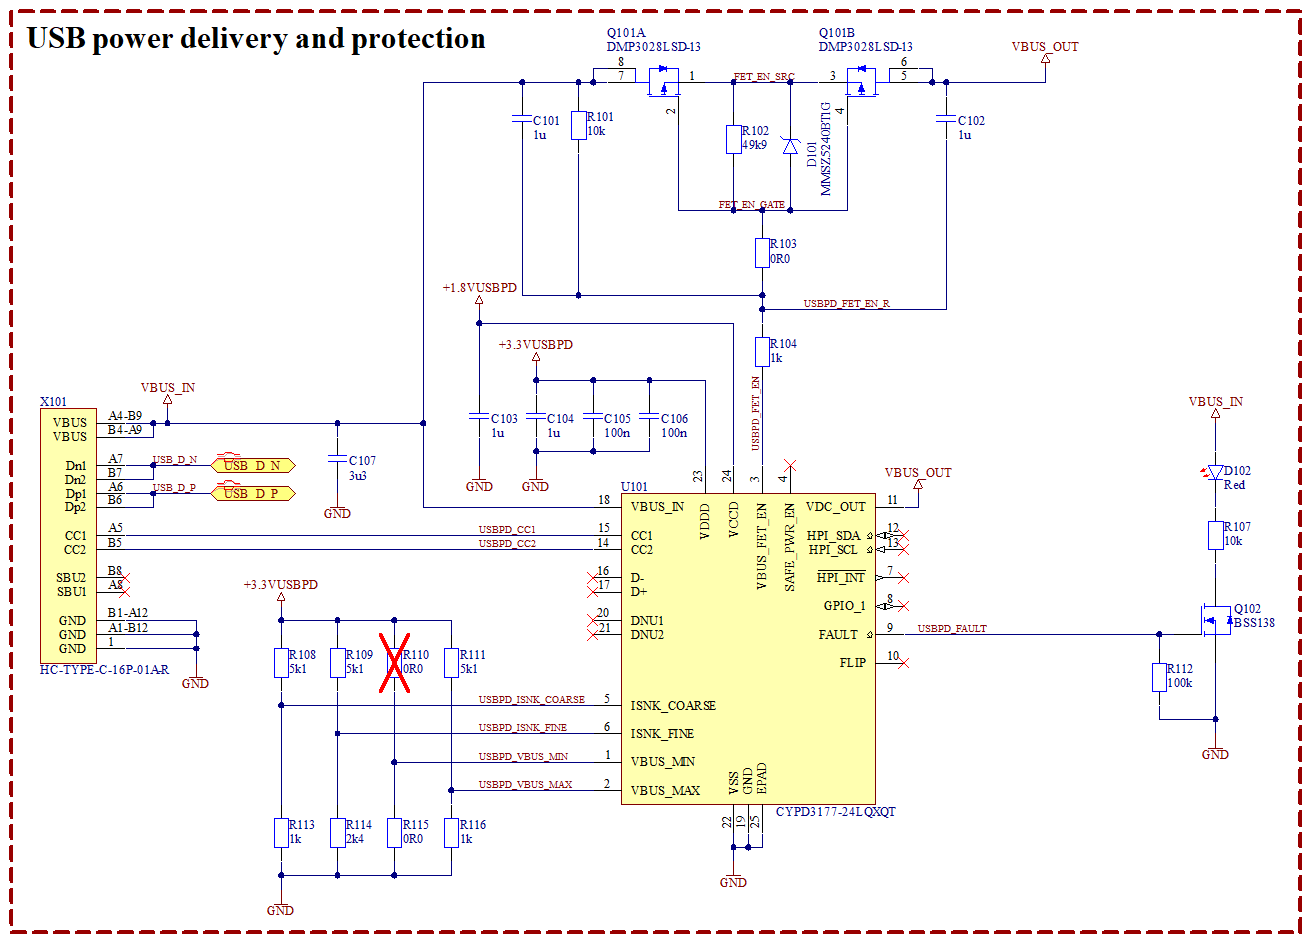
\includegraphics[width=\textwidth]{Figures/BR_USB.png}
    \caption{USB napajanje na narukvici}
    \label{slk:BR_USB}
\end{figure}
\section{PCB}
Tijekom projektiranja PCB osim što je bilo potrebno paziti na iste probleme kao i kod glavne ploče, bilo je potrebno paziti na ograničenje prostora i dvostranu montažu. Na slikama \ref{slk:BR_PCB_TOP} i \ref{slk:BR_PCB_BOT} prikazan je 3D prikaz projektiranje pločice.

Za razliku od glavne ploče, ovdje je podsustav za bežičnu komunikaciju postavljen tako da se antena nalazi u potpunosti izvan pločice. Tako će podsustav bolje primati signale i stvarati manje smetnje na pločicu tijekom slanja signala.

Ideja je da se PPG senzor nalazi na dijelu narukvice koja ostvaruje kontakt s kožom, pa je radi toga potrebno bilo postaviti senzor na donji sloj pločice (slika \ref{slk:BR_PCB_BOT}).

Radi ograničenja prostora maknute su sve testne točke i kratkospojnici.
\begin{figure}[htb]
    \centering
    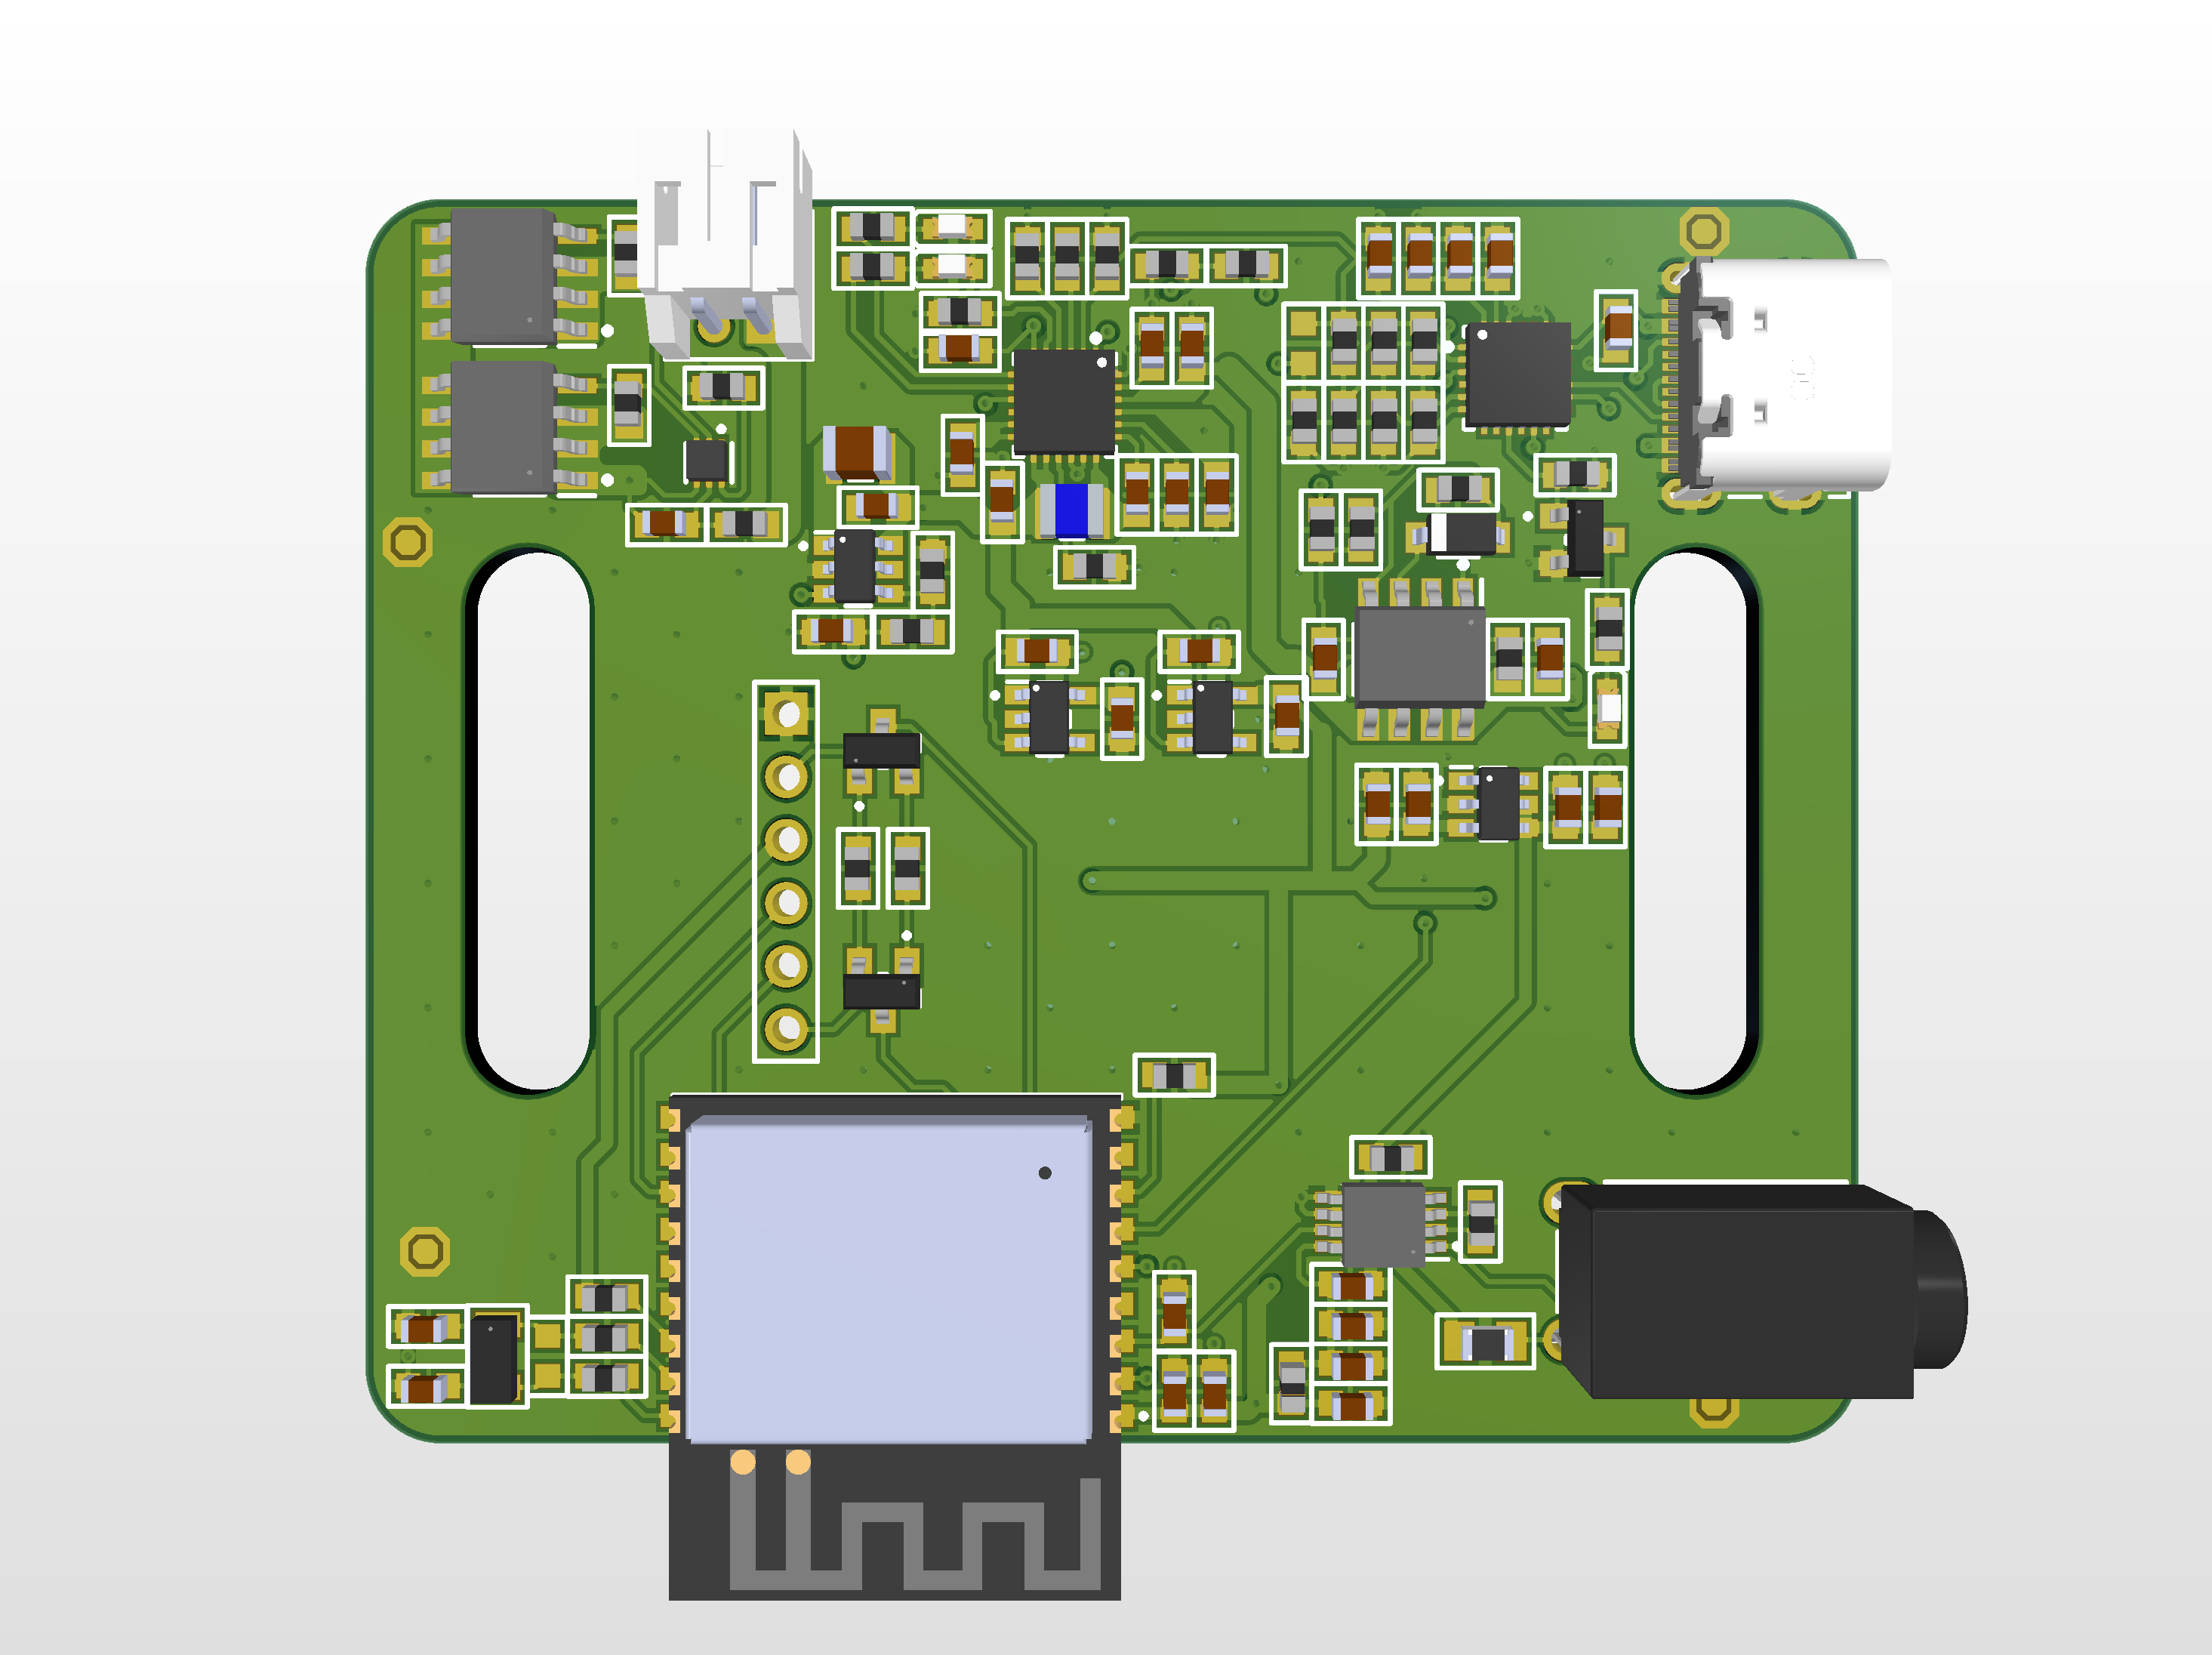
\includegraphics[width=10 cm]{Figures/BR_PCB.png}
    \caption{3D prikaz gornjeg sloja pločice}
    \label{slk:BR_PCB_TOP}
\end{figure}
\begin{figure}[htb]
    \centering
    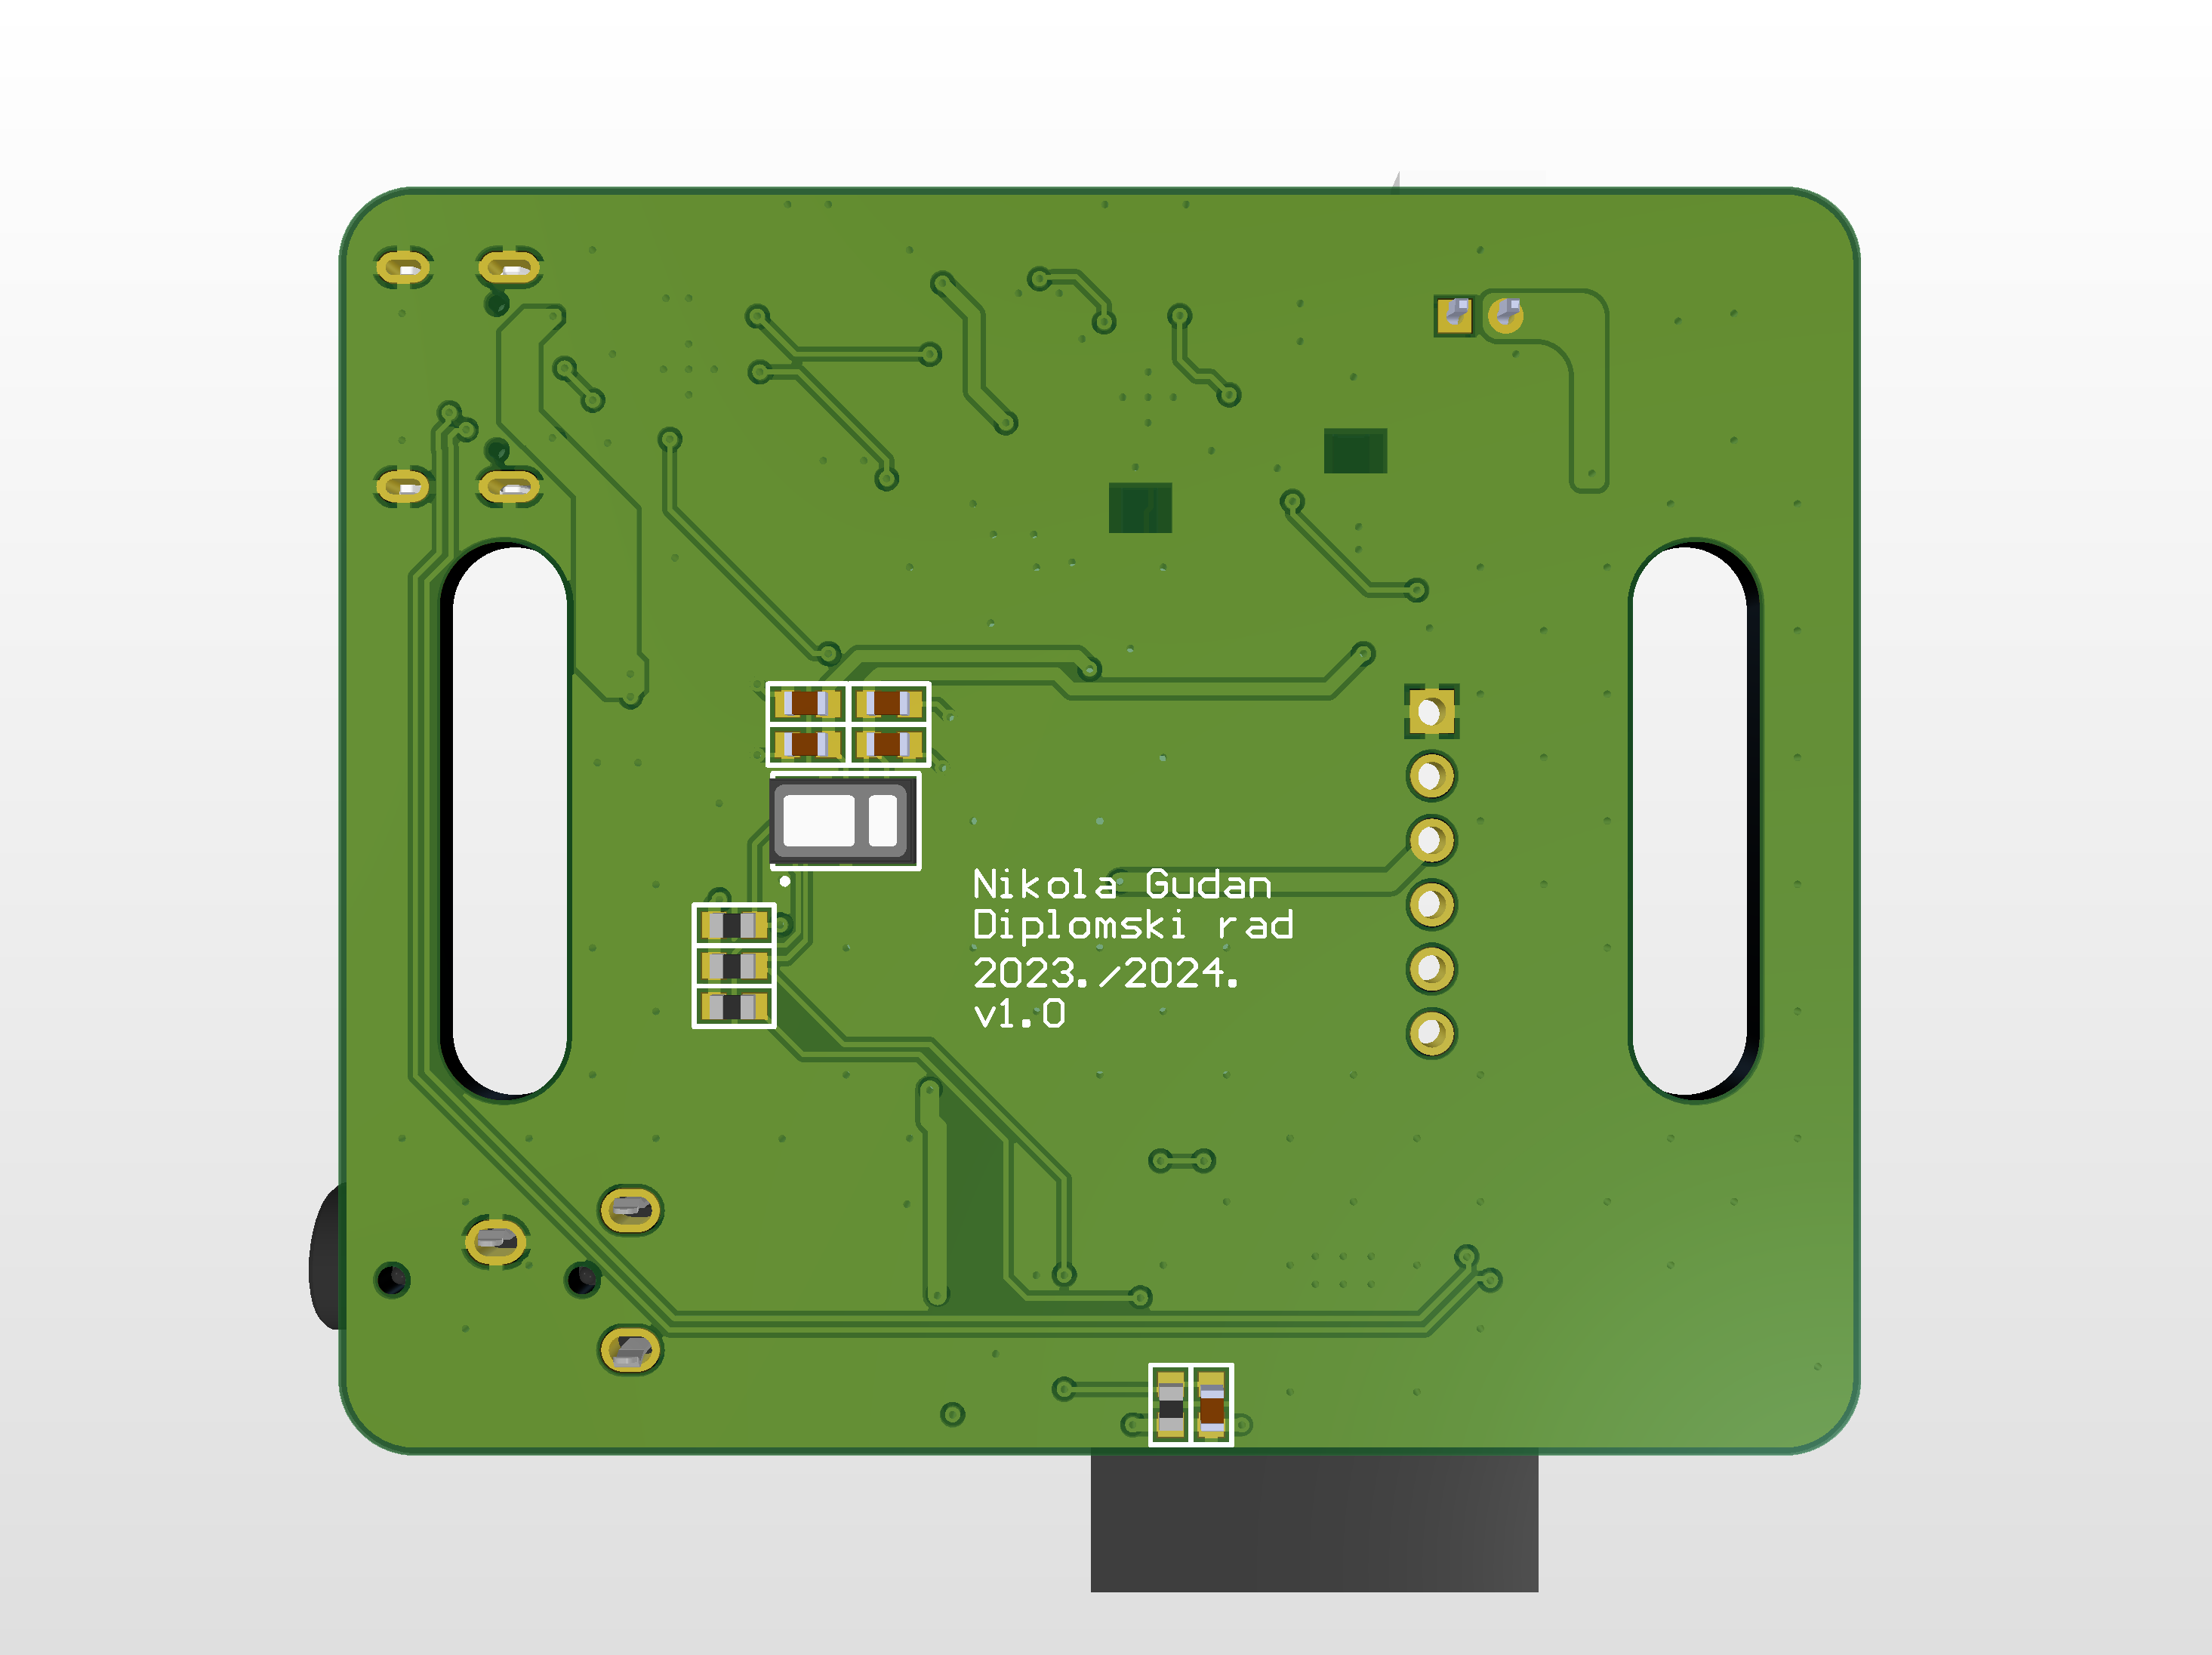
\includegraphics[width=10 cm]{Figures/BR_PCB_BOT.png}
    \caption{3D prikaz donjeg sloja pločice}
    \label{slk:BR_PCB_BOT}
\end{figure}